% Entorno

\section{Entorno}
	\subsection{¿Hay proyectos similares?}
	\begin{frame}
		\frametitle{¿Hay proyectos similares?}
		Si y no. \\
		Algunos proyectos similares:
		\setbeamercovered{invisible}
		\begin{itemize}
			\item <1-| alert@1> \url{http://www.cdlibre.org}
			\item <1-| alert@1> \url{http://www.osalt.com}
			\item <1-| alert@1> \url{http://winsol.uc3m.es}
			\item <1-| alert@1> \url{http://idefix.eup.uva.es/SLwin32/index.html}
			\item <1-| alert@1> \url{http://osluz.unizar.es/aplicaciones}
			\item <1-| alert@1> \url{http://crisol.uc3m.es/index.php/remository?func=select&id=1}
		\end{itemize}
	\end{frame}

	\begin{frame}
		\frametitle{Algunos proyectos similares}
		\begin{columns}
		\column{5.5cm}
			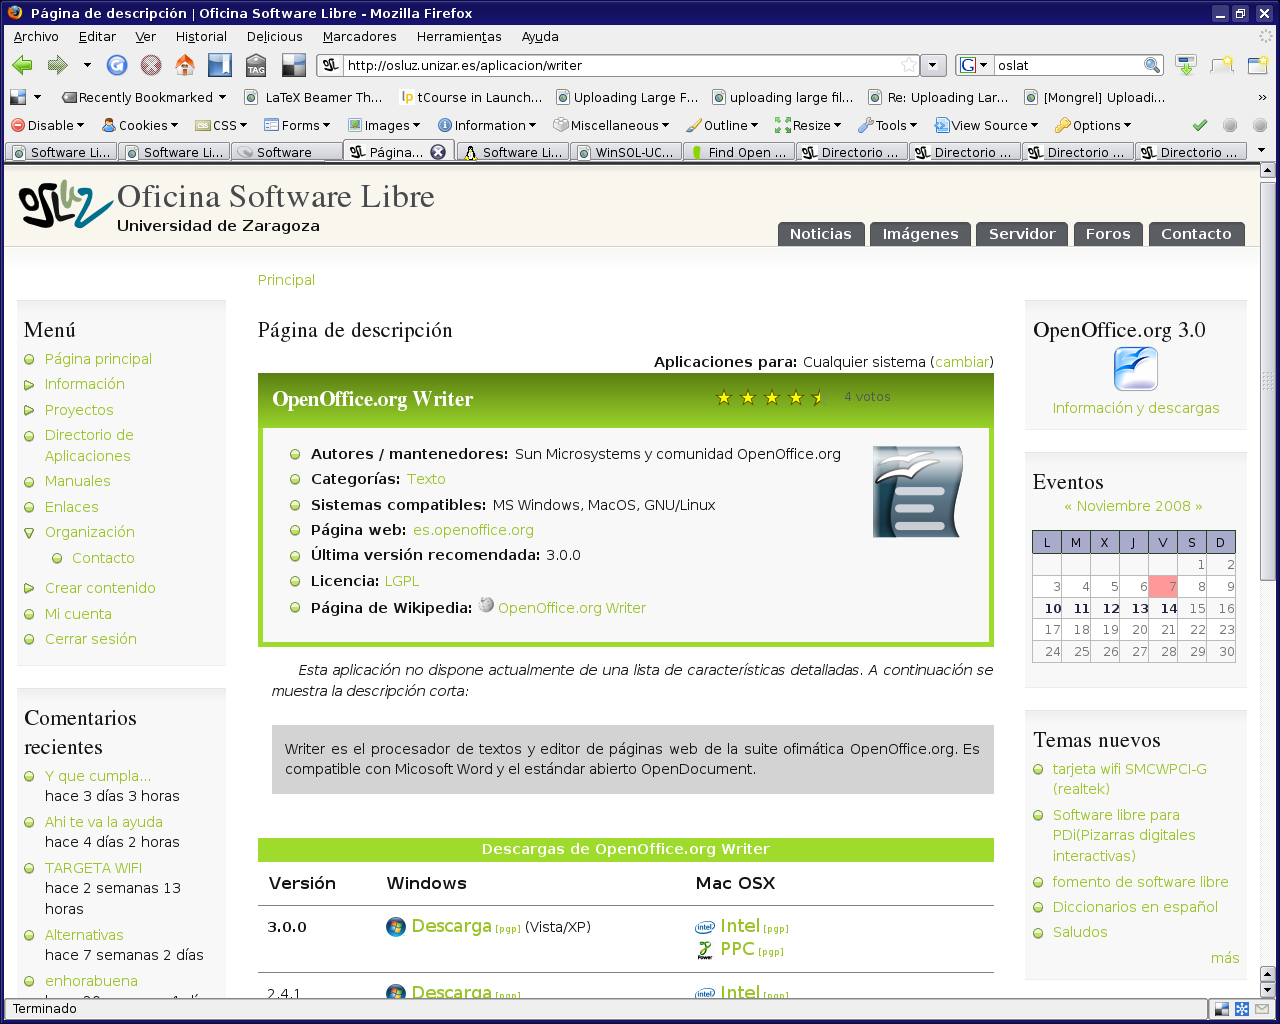
\includegraphics[width=2cm]{images/entorno01.png}
			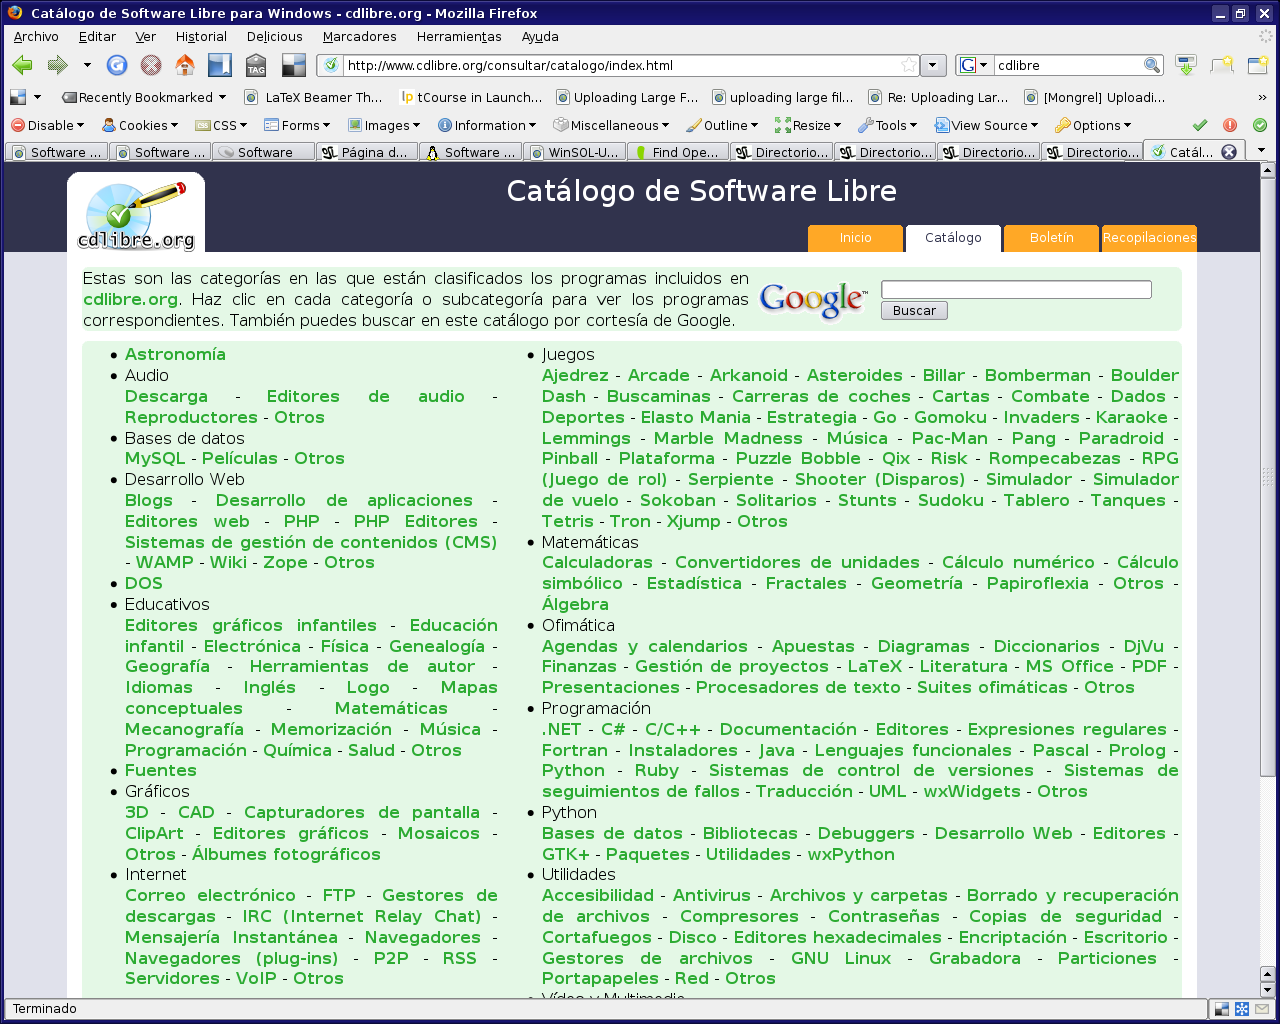
\includegraphics[width=2cm]{images/entorno02.png}
		\column{5.5cm}
			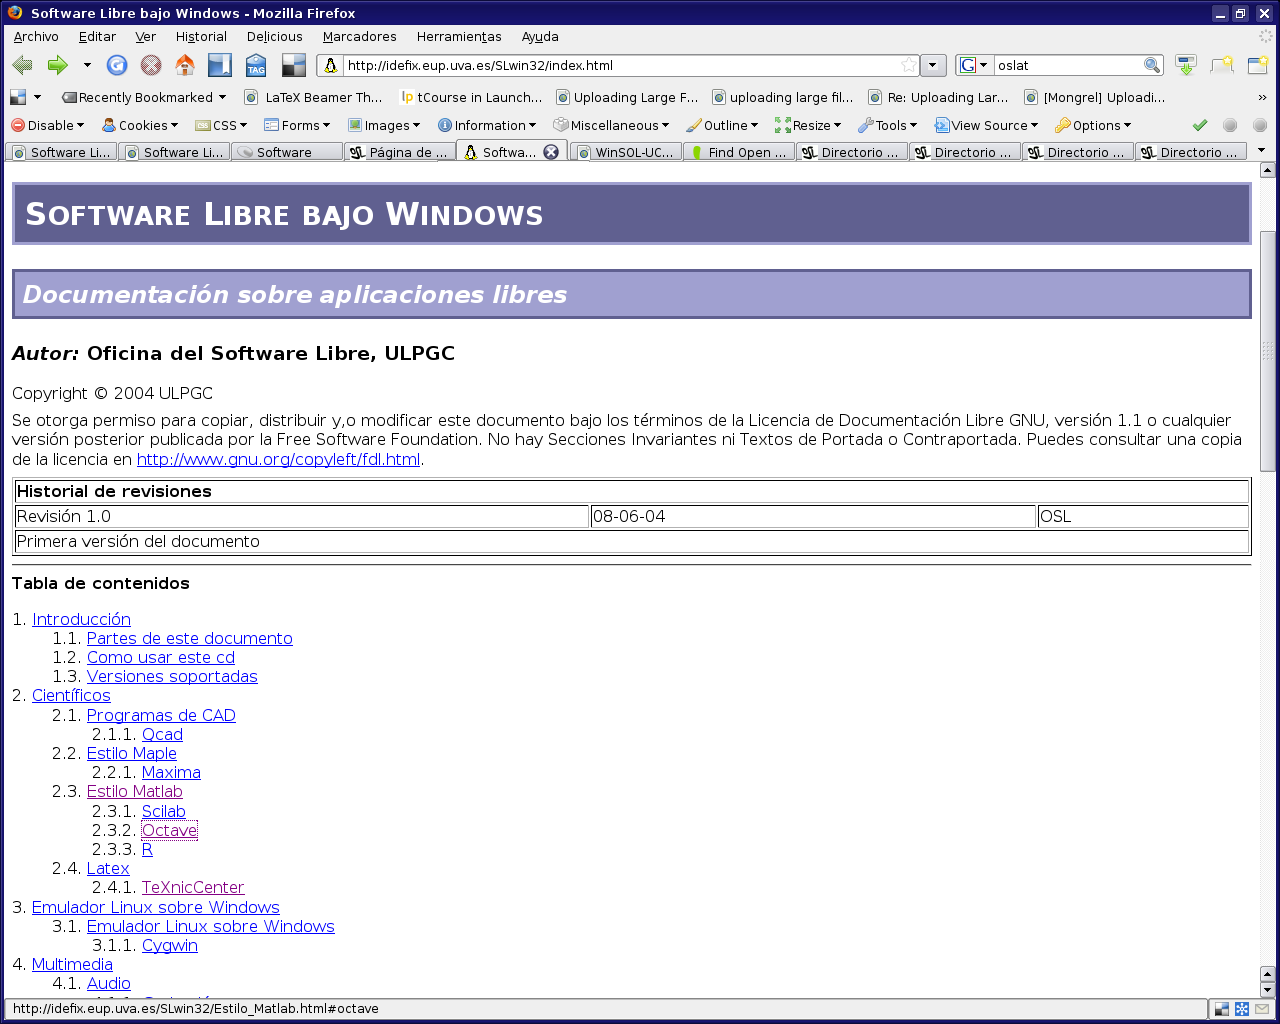
\includegraphics[width=2cm]{images/entorno03.png}
			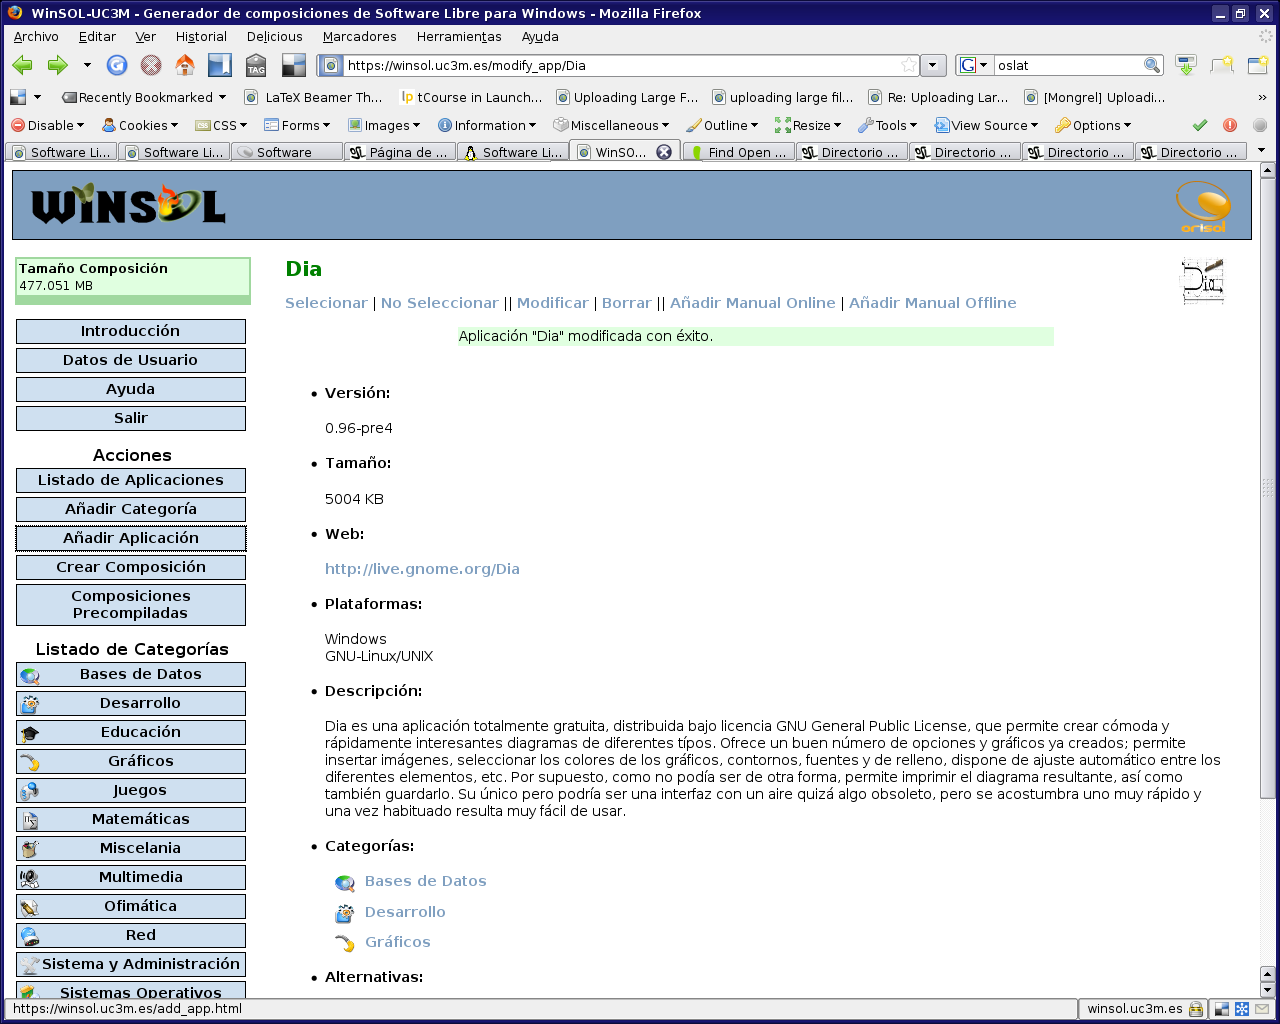
\includegraphics[width=2cm]{images/entorno04.png}
		\end{columns}
	\end{frame}

	
	\subsection{¿Qué ofrecen?} %que ofrecen otros
	\begin{frame}
		\frametitle{¿Qué ofrecen?}
		Es dificil generalizar porque son muy variadas las caracteristicas\ldtos
		\setbeamercovered{invisible}
		\begin{itemize}
			\item <1-| alert@1> Buenas catalogaciones
			\item <2-| alert@2> Contenidos de calidad y extensos
			\item <3-| alert@3> Buena información sobre las aplicaciones
			\item <4-| alert@4> Generación de imagen de CD para descargar
			\item <5-| alert@5> \ldots
		\end{itemize}
	\end{frame}

	\begin{frame}
		\frametitle{¿Qué NO ofrecen?}
		\setbeamercovered{invisible}
		\begin{itemize}
			\item <1-| alert@1> Equilibrio de todo lo anterior
			\item <2-| alert@2> Buscador de aplicaciones de calidad
			\item <3-| alert@3> Interactividad y participación del usuario
			\item <4-| alert@4> Sistemas de fidelización
			\item <5-| alert@5> \ldots
		\end{itemize}
	\end{frame}


	\subsection{¿Qué ofrecemos nosotros?} %porque nosotros somos mejores.
	\begin{frame}
		\frametitle{¿Qué ofrecemos nostros?}
		La creación de una comunidad \textbf{activa y participativa} de usuarios de software libre con gran cantidad de contenido, debidamente clasificado y altamente accesible, apoyado por la Oficina de Software Libre de la Universidad de La Laguna.

		Además el catalogo de software esta orientado a la comunidad universitaria, sin descuidadar al resto de potenciales usuarios.
	\end{frame}